\documentclass[12pt,a4paper]{article}

% Packages
\usepackage[utf8]{inputenc}
\usepackage[T1]{fontenc}
\usepackage[english]{babel}
\usepackage{amsmath,amssymb,amsfonts}
\usepackage{graphicx}
\usepackage{hyperref}
\usepackage{booktabs}
\usepackage{enumitem}
\usepackage{geometry}
\usepackage{natbib}
\usepackage{authblk}
\usepackage{xcolor}

% Provide \doi if not already defined by the bibliography style
\providecommand{\doi}[1]{\href{https://doi.org/#1}{doi:#1}}

\geometry{margin=2.5cm}

% Title
\title{\textbf{Intuitiveness as the Next Stage of Open Data: dataset design and complexity}}

% Authors
\author[a,d,*]{Sarazin Arthur}
\author[b,d]{Mourey Mathis}


\affil[a]{Researcher in Design Science, Veltys, France}
\affil[b]{Researcher in Data Science, The Hague University of Applied Sciences, Netherlands}
\affil[d]{Researcher associated with the UNESCO Chair ``AI and Data Science for Society''}

\vspace{1em}

\affil[*]{Corresponding author: asarazin@veltys.com}

\date{}

\begin{document}

\maketitle

%----------------------------------
% Abstract
%----------------------------------
\begin{abstract}
\textbf{Purpose:} Open data platforms face a critical challenge: datasets designed for expert users remain inaccessible to citizens and professionals with varying data literacy levels. This paper addresses the need for intuitive datasets whose complexity can adapt to user needs and capabilities, enabling broader value extraction from open data.

\textbf{Methods:} We develop a conceptual meta-design framework grounded in design science research methodology and hierarchical design patterns. The framework defines five data granularity levels (L0--L4), from atomic datums to unlinkable multi-level datasets. We formalise dataset complexity mathematically and demonstrate that transitions between granularity levels achieve 75--100\% complexity reduction. The framework is implemented as the open-source \texttt{intuitiveness} Python package, featuring AI-assisted entity discovery, semantic domain matching, and interactive navigation. We validate the approach through a case study with a major international logistics operator managing 8,368 indicators across multiple data sources.

\textbf{Results:} The descent phase (L4$\to$L0) transformed chaotic metadata into a clear atomic metric, revealing 40,279 relationships and enabling systematic identification of redundancy clusters. The ascent phase (L0$\to$L3) reconstructed intuitive multi-level tables that directly answered business questions about indicator consolidation. The accompanying Streamlit interface integrates with France's data.gouv.fr platform, making 45,000+ datasets accessible through guided workflows supporting both descent and ascent operations.

\textbf{Conclusions:} The framework provides a principled method for designing intuitive datasets that serve diverse data publics---from citizens seeking single facts to data scientists building complex products. By formalising complexity levels and reduction mechanisms, we enable open data platforms to move beyond one-size-fits-all presentations toward adaptive, user-responsive dataset designs. Future work includes formal user studies across literacy levels and extension to streaming data contexts.
\end{abstract}

\textbf{Keywords:} open data; meta-design; data literacy; framework; dataset complexity



%==================================
% SECTION 1: INTRODUCTION
%==================================
\section{Introduction}

\subsection{Context and motivation}

This conceptual meta-design framework aims at demonstrating how design can assist in producing useful open datasets and related data products. The framework and the associated package and interface (\textit{intuitiveness}) was created to support the open data community in their efforts to broaden the number of data publics \citep{ruppert2012} who use data to support decision-making, create new services and products, or produce innovative information and knowledge \citep{safarov2017}.

\subsection{Problem statement}

The conceptual meta-design framework meets the need for a method to design intuitive datasets, that is datasets whose shape can adapt to the data literacy level and the need of the user. There is a very diverse range of data users whose data literacy and needs differ greatly considering data: some will only look for one piece of information in the dataset while others will use data as a core artifact of a data product they are making. Yet, these diverse needs and data literacy levels have not been considered by open data producers while designing datasets \citep{dymytrova2018}.

\subsection{Contributions}

In this paper, we make the following contributions:
\begin{enumerate}
    \item We propose a conceptual meta-design framework based on five data granularity levels, enabling dataset designers to adapt complexity to user needs.
    \item We provide a formal definition of dataset complexity and demonstrate mathematically how transitions between granularity levels reduce complexity.
    \item We implement this framework as a Python library (\texttt{intuitiveness}) and validate it through a real-world case study with a major international logistics operator.
    \item We propose an interface that demonstrate the value of the \texttt{intuitiveness} package by making all CSVs files from the french public open data platform data.gouv.fr accessible to the package. 
    \item We offer practical guidelines for open data platforms to design intuitive datasets that address societal issues such as global warming, health, and public transparency.
\end{enumerate}

\subsection{Paper organisation}

The remainder of this paper is organized as follows. Section~\ref{sec:related-work} reviews related work on data literacy, open data reuse, and human-data interaction. Section~\ref{sec:framework} presents our conceptual meta-design framework with five granularity levels. Section~\ref{sec:complexity} provides the formal complexity analysis. Section~\ref{sec:case-study} describes the implementation and case study. Section~\ref{sec:discussion} discusses implications and limitations. Finally, Section~\ref{sec:conclusion} concludes the paper and outlines future work.

%==================================
% SECTION 2: RELATED WORK
%==================================
\section{Related Work}
\label{sec:related-work}

Our work on intuitive datasets draws from several research streams: adaptive data visualisation, user modelling and assessment, documentation design, and human-data interaction. We review each in turn, highlighting how existing approaches inform our meta-design framework.

\subsection{Adaptive data visualisation}

A growing body of research addresses the challenge of adapting visualisations to users with varying levels of expertise. \citet{poetzsch2020towardataxonomy} propose a taxonomy for adaptive data visualisation in analytics applications, distinguishing between user traits (e.g., statistical expertise, graphical literacy) and user states (e.g., monitoring vs. analysis tasks). Their empirical evaluation reveals that monitoring tasks with higher data complexity receive better suitability ratings, while analysis tasks require richer interactive features such as filtering, brushing, and drill-down capabilities. This suggests that different granularity levels may be appropriate for different analytical intents---a principle we formalise in our framework.
\vspace{1em}
\noindent \citet{steichen2013useradaptiveinformationvisualisation} demonstrate that eye gaze data can predict users' current visualisation tasks and cognitive abilities, including perceptual speed, visual working memory, and verbal working memory. Their work enables real-time adaptive interventions such as highlighting relevant elements or de-emphasizing non-relevant data to reduce cognitive load. Notably, they find that users with low perceptual speed particularly benefit from adaptive assistance, reinforcing the need for interfaces that can dynamically adjust complexity.

\vspace{1em}

\noindent \citet{amyrotos2021adaptivevisualisationsfor} critiques the prevalent ``one-size-fits-all approach'' in data visualisation tools and proposes a human-centered adaptive visualisation framework. This framework incorporates a multi-dimensional user model considering cognitive factors, domain expertise, and task context. A data visualisation engine then recommends best-fit visualisations, while an intelligent analytics component continuously refines the user model through interaction tracking. This work underscores the importance of moving beyond static dataset presentations toward dynamic, user-responsive designs.

\subsection{Visualisation recommenders and progressive disclosure}

Selecting appropriate visualisations poses significant challenges for non-expert users. \citet{mutlu2016vizrec} address this through VizRec, a recommender system that suggests personalized visualisations by combining perceptual guidelines with user preferences. The system uses tag vectors to describe visualisation content for content-based filtering and quality ratings for collaborative filtering. By reducing combinatorial explosion through perceptual constraints, VizRec alleviates choice overload---a key barrier to data accessibility for users with limited visualisation literacy.

\vspace{1em}

\noindent \citet{cockburn2014supportingnoviceto} examine the broader challenge of supporting novice-to-expert transitions in user interfaces. They document systems like FollowUs, which integrates online tutorials within applications and enables community contributions, leading to higher task completion and lower frustration. The Chronicle system visualizes user workflows via a zoomable timeline, supporting reflection on interaction strategies. These mechanisms for progressive skill development complement our approach of progressive complexity reduction.

\subsection{Dashboard Design and User-Centered Challenges}

\noindent \citet{alhamadi2022dataqualitymismatched} provide empirical insights into the challenges of user-centered dashboard design. Through interviews with dashboard developers, they identify a significant gap between users' visual literacy and dashboard requirements. Their work categorizes three adaptation mechanisms: \textit{customization} (user-initiated modifications), \textit{personalization} (system-driven adjustments at load time), and \textit{automatic adaptation} (real-time updates based on user models). Developers report implementing practices such as minimal default charts, consistent color schemes, role-tailored filters, and explicit interpretation of visualisations.

\vspace{1em}

\noindent Crucially, \citeauthor{alhamadi2022dataqualitymismatched} find that users often struggle not only with visualisation complexity but also with understanding data provenance and trusting displayed information. They recommend layered documentation---high-level summaries, in-situ definitions, and links to machine-readable metadata---to address these concerns. This resonates with our goal of designing datasets whose structure can reveal or hide complexity based on user needs.

\subsection{User Modeling and Literacy Assessment}

\noindent Effective adaptation requires accurate assessment of user capabilities. \citet{steichen2013useradaptiveinformationvisualisation} pioneer the use of behavioural telemetry for user modelling, demonstrating that gaze patterns can infer cognitive abilities with accuracy significantly above baseline. Prior work they reference shows that mouse click behaviour and visualisation selections can reveal user expertise and suboptimal usage patterns.

\vspace{1em}

\noindent \citet{amyrotos2021adaptivevisualisationsfor} extends this with reflective analytics and learning-curve modelling to refine user models over time. The goal is a ``generic data visualisation engine'' that renders appropriate visualisations based on data characteristics, user models, and task specifications. Such systems move toward the vision of intuitive datasets that automatically calibrate their presentation to each user's proficiency level.

\subsection{Positioning Our Contribution}

\noindent Existing work focuses predominantly on adapting \textit{visualisations} and \textit{interfaces} to user characteristics. However, comparatively little attention has been paid to adapting the \textit{underlying dataset structure} itself. Our framework addresses this gap by proposing that datasets can be designed with multiple granularity levels, enabling not just different visual presentations but fundamentally different data structures optimised for users at different literacy levels.

\vspace{1em}

\noindent While adaptive visualisation systems adjust how data is shown, our approach adjusts what data is shown and how it is organized. This represents a shift from presentation-layer adaptation to data-layer adaptation. By formalising complexity levels and reduction mechanisms, we provide dataset designers with a principled method for creating intuitive open datasets that can serve diverse data publics---from citizens seeking a single fact to data scientists building complex products.

%==================================
% SECTION 3: CONCEPTUAL FRAMEWORK
%==================================
\section{Conceptual Meta-Design Framework}
\label{sec:framework}

To create the conceptual meta-design framework we used the design science research methodology \citep{hevner2004} and applied the Hierarchical design pattern \citep{vaishnavi2015}. This pattern uses the divide and conquer strategy to design a complex system. It designs a system (the conceptual meta-design framework) by decomposing it into subsystems (five conceptual design frameworks to design each of the five granularity levels of one dataset), designing each of them before designing the interactions between them.

\vspace{1em}

\noindent We also ensured, following the recursive principle of granular computing that secures a high level of human-data interaction \citep{wilke2016}, that datasets of an upper granularity level could be constructed by human extrapolation of datasets of lower granularity levels.

\vspace{1em}

\noindent We consider five \emph{data granularity levels} for every dataset, hence five conceptual design frameworks. By \emph{data granularity level} we mean the size of the informational unit treated as a single object in a representation: a value (L0), a vector (L1), a table (L2), a linked graph (L3), or an unlinked collection of artefacts (L4). The term is drawn from the granular-computing tradition \citep{wilke2016}, where granules are the elementary units of human--data interaction. We prefer it to the more common ``level of data abstraction'' because the latter is heavily overloaded in computer science---denoting variously the interface-hiding of abstract data types in object-oriented programming, the view layers of the ANSI/SPARC database architecture, category formation in artificial intelligence and knowledge representation, and the task-driven re-description of datasets in visualisation research---none of which coincides with the granularity hierarchy we describe.

\vspace{1em}

\noindent At the highest level, \textbf{Level 4} encompasses data made of unlinkable and multi-level datasets. Descending to \textbf{Level 3}, we find data made of linkable and multi-level datasets. \textbf{Level 2} represents data made of a single dataset with several entities and attributes. Moving further down, \textbf{Level 1} consists of data made of a single entity and several attributes, or alternatively of a single attribute and several entities. Finally, at the most granular level, \textbf{Level 0} comprises data made of a single entity, a single attribute, and a single value---corresponding to the classical definition of data as a triplet entity-value-attribute \citep{redman1997}, also considered as the fundamental information granule.

\noindent These five levels were designed according to the five stages of an intuitive process \citep{csikszentmihalyi1997flow}. \textbf{Level 0} corresponds to the preparation stage, where the user becomes interested in some datum (for example, discovering that 65 percent of the population uses chatGPT on a daily basis). \textbf{Level 1} corresponds to the incubation stage, where the user unfolds the datum and makes unusual connections (for instance, hypothesizing that the people using chatGPT on a daily basis should be the youngest). \textbf{Level 2} corresponds to the insight stage, where the user starts to put pieces together (such as comparing the 'age' and the 'daily gpt use' columns inside a data table to see if there is a pattern between the two). \textbf{Level 3} corresponds to the evaluation stage, where the user puts their insight on trial (for example, the user challenges their intuition that people using chatGPT must be the youngest by collecting a different dataset with the probability of being a chatGPT daily user depending on age class). Finally, \textbf{Level 4} corresponds to the elaboration stage where the user will use other logical mechanisms than data aggregation to make sense of different datasets (for instance, the user might look for demographic distributions to see what proportion the youngest represent out of an entire population and then specify that if 65 percent of the population are daily users of chatGPT, the users are mostly the youngest, showing the technology has not spread yet to the entire population).

\vspace{1em}

\noindent According to these definitions, data will be qualified as intuitive if it allows to go up the level ladder in order to elaborate from a single value or, in the opposite direction, go down the level ladder to unconver an insight that will trigger curiosity or decision-making.

\vspace{1em}

\noindent To name what is at stake at each step, we adopt the vocabulary of Bruno Latour's analysis of scientific reference \citep{latour1999}. In \textit{Pandora's Hope}, Latour shows that every link in a chain of reference performs a controlled trade: a \textbf{reduction} of one property of the represented world is exchanged for an \textbf{amplification} of another. Travelling down a chain (a sample of soil becomes a labelled jar, then a colour-coded chart, then a number in a report) trades situatedness for transferability; travelling up reverses the trade. The descent phase of our framework is, in these terms, a chain of four reductions, each one purchasing a specific amplification:
\begin{itemize}[leftmargin=2em,itemsep=0.2em]
\item L4$\to$L3 reduces \textit{artefactual heterogeneity} in exchange for \textit{relational structure};
\item L3$\to$L2 reduces \textit{domain breadth} in exchange for \textit{domain coherence};
\item L2$\to$L1 reduces \textit{attribute dimensionality} in exchange for \textit{feature legibility};
\item L1$\to$L0 reduces \textit{observational extent} in exchange for \textit{atomic certainty}.
\end{itemize}
The ascent phase reverses the polarity, chaining three amplifications that repay what was bought during the descent:
\begin{itemize}[leftmargin=2em,itemsep=0.2em]
\item L0$\to$L1 amplifies \textit{variation along a dimension} at the cost of atomic isolation;
\item L1$\to$L2 amplifies \textit{attribute coverage} at the cost of feature isolation;
\item L2$\to$L3 amplifies \textit{inter-domain linkage} at the cost of domain isolation.
\end{itemize}
Under this vocabulary, the user is not ``navigating'' through a fixed space but engaging in a sequence of \emph{deliberate commitments}: each transition is a contract whose terms can later be renegotiated. ``Intuitive data'' is then data for which both directions of the chain---reductions and amplifications---can be traversed without loss of provenance, so that every commitment made at a transition remains visible, comparable across alternatives, and reversible.

\vspace{1em}

\noindent All in all, this paper sets forth a meta-design framework that will enable data modelers, architects, analysts and data platform editors to put data users in a position of experiencing the "flow", that is a mental state "expected to occur when individuals perceive greater opportunities for action than they encounter on average in
their daily lives, and have skills adequate to engage them" \citep{nakamura2014concept}


%----------------------------------
% Subsection 3.1: Level 0
%----------------------------------
\subsection{Level 0: The Datum}

\noindent Data made of a single entity, attribute, and value corresponds in our framework to a Level 0 dataset, with no complexity. It can also be referred to as a ``datum.'' A datum is defined as the smallest informational granule or the fundamental particle of data science. In computer science, the datum is defined as a triple entity-attribute-value. It can be represented by a table with a single cell (see Figure~1).

\begin{figure}[h!]  % h = here, ! = force it
    \centering
    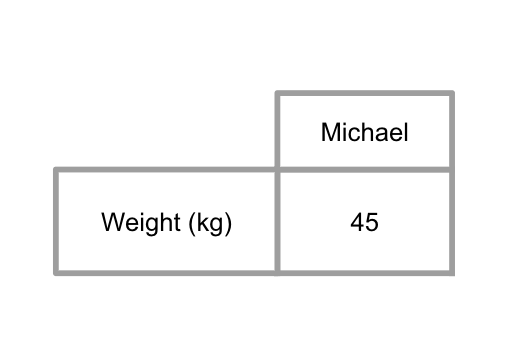
\includegraphics[width=0.4\linewidth]{0.png}
    \caption{Table view of Level 0 data}
    \label{fig:placeholder}
\end{figure}

\noindent At the lowest granularity level, Level 0, data has no complexity as no interpretation is required for its comprehension. This type of data is commonly referred to as ``raw data.'' For instance, in our example, Michael weighs 45~kg, which is a fact.

%----------------------------------
% Subsection 3.2: Level 1
%----------------------------------
\subsection{Level 1: Single Entity or Single Attribute}

To move from Level 0 to Level 1 of granularity, we need to find a common element among several data. It can be a common attribute (`weight'), a common entity (`Michael'), or a common value. As a result, we can obtain a table with a single entity defined by multiple attributes, or a table with a single attribute and multiple entities (see Figure~2). These tables are the primary form of what we call `data' (plural of `datum').

\begin{figure}[h!]  % h = here, ! = force it
    \centering
    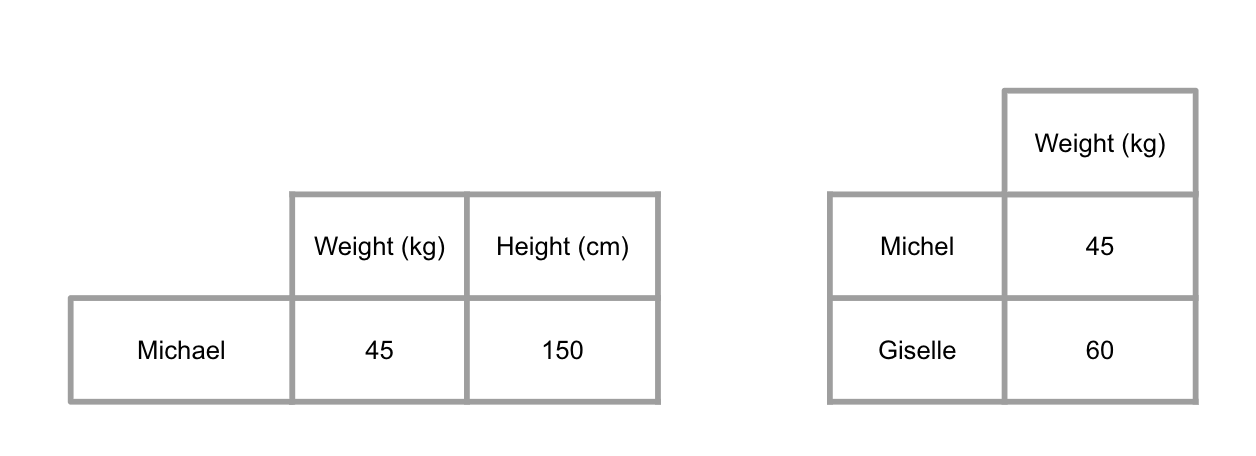
\includegraphics[width=0.8\linewidth]{1.png}
    \caption{Table view of two Level 1 data}
    \label{fig:placeholder}
\end{figure}



%----------------------------------
% Subsection 3.3: Level 2
%----------------------------------
\subsection{Level 2: Single Dataset with Multiple Entities and Attributes}

To increase complexity and move from Level 1 to Level 2, it logically involves adding attributes and/or entities to the table (see Figure~3).

\begin{figure}[h!]  % h = here, ! = force it
    \centering
    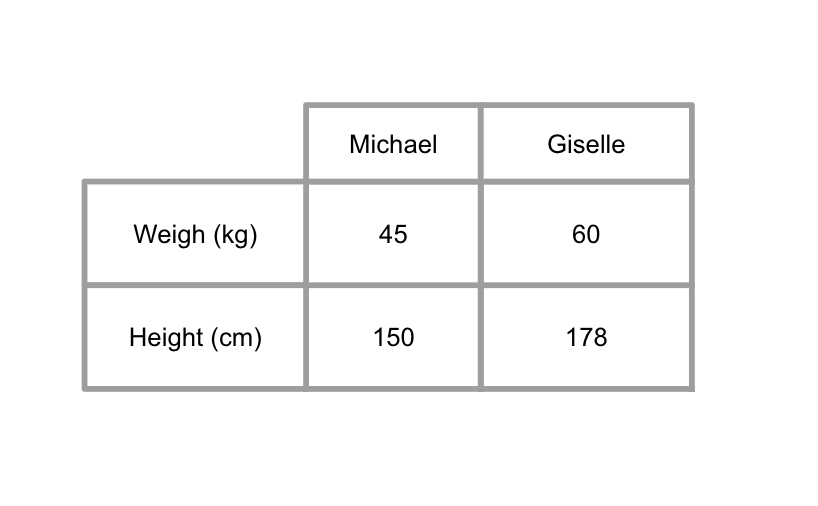
\includegraphics[width=0.5\linewidth]{2.png}
    \caption{Table view of Level 2 dataset}
    \label{fig:placeholder}
\end{figure}

%----------------------------------
% Subsection 3.4: Level 3
%----------------------------------
\subsection{Level 3: Linkable Multi-Level Datasets}

At a higher granularity level, data transition from one to many linkable datasets and from one to many levels of entities and/or attributes. This results in linkable datasets, consisting of multiple levels of entities and multiple levels of attributes (see Figure~4).

\begin{figure}[h!]  % h = here, ! = force it
    \centering
    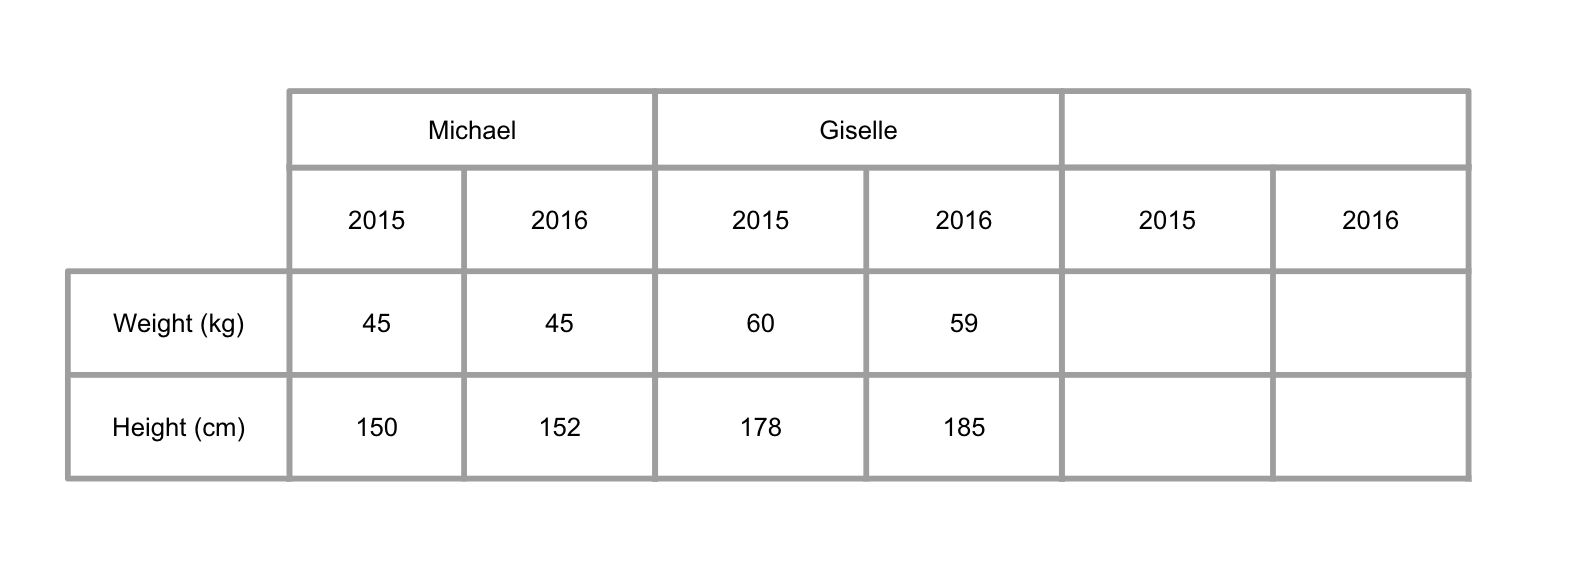
\includegraphics[width=0.7\linewidth]{3.png}
    \caption{Table view of Level 3 multi-level dataset with two entity dimensions (individuals, years) and one attribute dimension (physical characteristics)}
    \label{fig:placeholder}
\end{figure}

In the above example, we have two levels of entities: individuals on one side, and years on the other. We also have one level of attribute: individual physical characteristics (weight and height).


%----------------------------------
% Subsection 3.5: Level 4
%----------------------------------
\subsection{Level 4: Unlinkable Multi-Level Datasets}

At the highest granularity level, data transition from definable complexity to undefinable complexity. These are multi-level data tables that cannot be linked based on current scientific knowledge. These multi-level tables are characterized by the fact that their junction cannot be represented in the form of tables, since their level of complexity is indefinable. At best, they could be represented by a disconnected graph. 

\vspace{1em}

\noindent It has become commonplace to state that there is an ever-increasing amount of data available, which implies an underlying structure of extreme intelligence that can link data together. This structure would enable the discovery of fascinating knowledge and the creation of innovative applications. In this article, we assume that the reality of newly available data is quite different: there is no apparent structure to link them together, or if it does exist, it is indefinable based on current scientific knowledge. From our conceptual meta-design framework's perspective, all newly available datasets are Level 4 data.

Indeed, the available data, in their vast majority, do not share any attributes or common elements that would allow them to be linked together. For example, the link between daily shopping baskets in supermarkets and monthly water consumption in surrounding households has not been established. It may not exist, but certainly the complexity of the link is indefinable based on current scientific knowledge.

\subsection{Summary}

We have shown in this section that data can be represented according to five granularity levels. Level 0 and Level 4 are purely theoretical in nature, being respectively the domain of machines and human beings. Our main focus is to establish the conceptual framework of intuitive data, which are defined as data whose granularity level and complexity can adapt to the data literacy level of the user.

In the following section, we formally demonstrate that transitioning from a higher granularity level to a lower level decreases the complexity of the data, and we determine to what extent this complexity decreases.

%==================================
% SECTION 4: FORMAL COMPLEXITY ANALYSIS
%==================================
\section{Formal Complexity Analysis}
\label{sec:complexity}

\subsection{Definition of Dataset Complexity}

The complexity of a dataset can be measured by the number of relationships that can be extracted from it. In this framework, we consider that the order of complexity ($C()$) associated with a dataset relates to how fast the complexity increases with the size of the dataset.

Let us consider the derivation of the order of complexity for each level:

\paragraph{Level 0:}
The complexity of a single data point is equal to zero. There is no complexity associated with a single point of information. The order of complexity is $C(0)$.

\paragraph{Level 1:}
For a variable or a single vector of values, there is only one way to interpret the data: we look at how all data points compare to each other. Since there is only one way to look at the data, the order of complexity is $C(1)$.

\paragraph{Level 2:}
For a (single-level) table, we can consider the following: (1) we can interpret each row/column independently; (2) we can combine one row (or column) with one or more rows (or columns) to study the relationship they have.

The overall number of combinations we can make in a table with $n$ rows is: $2^n - 1$. We define the order of complexity as how fast the complexity grows with each new row:
\begin{equation}
2^{n+1} - 1 - (2^n - 1) = 2^{n+1} - 2^n = 2^n (2 - 1) = 2^n
\end{equation}
The order of complexity is: $C(2^n)$.

\paragraph{Level 3:}
For a multi-level table, the complexity depends on the number of rows/columns ($n$) and the number of groups for each level ($g$). The total number of possible combinations is: $2^{ng} - 1$.

Considering the growth of complexity when adding a new group:
\begin{equation}
2^{n(g+1)} - 1 - (2^{ng} - 1) = 2^{n(g+1)} - 2^{ng} = 2^{ng} (2^n - 1)
\end{equation}
The order of complexity is: $C(2^{ng}(2^n - 1))$.

\paragraph{Level 4:}
Unlinkable tables correspond to infinite complexity: $C(\infty)$.

\subsection{Complexity Reduction}

We examine how to reduce the order of complexity by transforming a higher level into a lower one. The closed-form bounds below quantify the \emph{reduction} side of each descent transition---how much complexity is shed when moving from one level to the next. In the vocabulary of \S\ref{sec:framework}, each numerical $\Delta C$ must be read against the qualitative \emph{amplification} it purchases (relational structure at L4$\to$L3, domain coherence at L3$\to$L2, feature legibility at L2$\to$L1, atomic certainty at L1$\to$L0), which the framework articulates but does not attempt to quantify here. We consider single-level reductions and measure the relative reduction:
\begin{equation}
\Delta C = \frac{C_{\text{after}} - C_{\text{before}}}{C_{\text{before}}}
\end{equation}

\subsubsection{Level 4 to Level 3 — reduction of artefactual heterogeneity}
Going from an infinitely complex dataset to a measurably complex dataset is, by definition, an almost perfect reduction of complexity. The amplification purchased by this reduction is \emph{relational structure}: previously unlinkable artefacts acquire a shared entity model.

\subsubsection{Level 3 to Level 2 — reduction of domain breadth}
For the upper bound:
\begin{equation}
\Delta C = \lim_{g \to \infty} \frac{2^n - 2^{ng}(2^n - 1)}{2^{ng}(2^n - 1)} = -100\%
\end{equation}

For the lower bound (simplest Level 3: $g=2$, $n=2$):
\begin{equation}
\Delta C = \frac{1}{2^{2(2-1)}} - 1 = \frac{1}{4} - 1 = -75\%
\end{equation}

The reduction is bounded: $\Delta C \in [-100\%; -75\%]$. The amplification purchased here is \emph{domain coherence}: the multi-entity graph is partitioned into a single domain-scoped table.

\subsubsection{Level 2 to Level 1 — reduction of attribute dimensionality}
\begin{equation}
\Delta C = \lim_{n \to \infty} \frac{1 - 2^n}{2^n} = -100\%
\end{equation}

For the lower bound (simplest Level 2: $n=2$):
\begin{equation}
\Delta C = \frac{1}{2^2} - 1 = -75\%
\end{equation}

The reduction is bounded: $\Delta C \in [-100\%; -75\%]$. The amplification purchased here is \emph{feature legibility}: a single attribute (or entity) is isolated as the analytical focus.

\subsubsection{Level 1 to Level 0 — reduction of observational extent}
\begin{equation}
\Delta C = \frac{0 - 1}{1} = -100\%
\end{equation}

Any complexity reduced to Level 0 corresponds to a 100\% reduction. The amplification purchased here is \emph{atomic certainty}: the feature vector collapses to a single value with the highest possible transferability across contexts.

%==================================
% SECTION 5: CASE STUDY
%==================================
\section{Case Study and Implementation}
\label{sec:case-study}


We implemented this method in a Python library (\texttt{intuitiveness}), applied it to a dataset from a major international logistics operator and developed an interface. 

\subsection{Case study}

\subsubsection{Problem context}
The organisation faced an overwhelming amount of metadata on their indicators, coming from different sources and formats, making it difficult to manage their data ecosystem effectively. Their core challenge was: \textbf{given these metadata, how to identify which indicators to delete for operational efficiency while maintaining analytical capabilities?} With 8,368 indicators scattered across multiple sources, there was no intuitive way to determine which were essential and which were redundant or obsolete.

\subsubsection{The Descent Phase (L4 $\to$ L0)}

\vspace{1em}

\noindent {Step 1: L4 $\to$ L3 (Graph Construction)}
We modeled the raw ``unlinkable'' files into a knowledge graph, transforming a Level 4 dataset into Level 3. The graph revealed 40,279 relationships among 8,368 indicators (48 connections per indicator on average).

\vspace{1em}

\noindent {Step 2: L3 $\to$ L2 (Domain Isolation)}
We queried the graph to isolate indicators by domain: revenues, volumes, and employees (ETP). This categorical structure provided the first layer of intuitive organisation.

\vspace{1em}

\noindent {Step 3: L2 $\to$ L1 (Feature Extraction)}
We extracted indicator names to analyse naming conventions and identify duplicates.

\vspace{1em}

\noindent {Step 4: L1 $\to$ L0 (Atomic Metric)}
We derived the atomic metric: \textit{number of revenue indicators}. This precise formulation captures a business diagnostic---an overproduction of indicators---and served as the ground truth for the audit.

\vspace{1em}


\subsubsection{The Ascent Phase (L0 $\to$ L3)}

\vspace{1em}

\noindent {Step 5: L0 $\to$ L1 (Reconstructing the Vector)}
From the atomic metric, we reconstructed a vector of naming signatures by extracting structural features from each indicator name.

\vspace{1em}

\noindent {Step 6: L1 $\to$ L2 (Initial Classification)}
We added categories to the indicators. The \texttt{business\_objects} category captures the business domain (volume, revenue, ETP). The \texttt{calculated} category provides a binary flag distinguishing raw data from calculated metrics. We also introduced three binary flags: \texttt{weight\_flag}, \texttt{rse\_flag}, and \texttt{surcharges\_flag} to capture specific business attributes.

\vspace{1em}

\noindent {Step 7: L2 $\to$ L3 (Analytic Dimensions)}
We added analytic dimensions to enable multi-level analysis. The \texttt{client\_segmentation} dimension specifies which client segments are addressed. The \texttt{sales\_location} dimension captures geographic usage patterns. The \texttt{product\_segmentation} dimension identifies which products are included. The \texttt{financial\_view} dimension provides the financial perspective of the indicator. Finally, the \texttt{lifecycle\_view} dimension indicates the business lifecycle stage being measured.

\subsubsection{Results}

The \textbf{descent} (L4 $\to$ L0) moved the organisation from chaos to a clear atomic metric. The \textbf{ascent} (L0 $\to$ L3) produced intuitive Level 3 tables answering the business question.

The Level 3 table reveals clusters of indicators sharing identical analytic dimensions:

\begin{table}[h]
\centering
\small
\begin{tabular}{@{}lllllll@{}}
\toprule
\textbf{Indicator} & \textbf{Object} & \textbf{Client} & \textbf{Location} & \textbf{Product} & \textbf{Financial} & \textbf{Lifecycle} \\ \midrule
\texttt{CA|4p|12caps} & revenue & All & Global & All & operational & current \\
\texttt{CA|4p|11caps} & revenue & All & Global & All & operational & current \\
\texttt{CA|4p|10caps} & revenue & All & Global & All & operational & current \\ \bottomrule
\end{tabular}
\caption{Example of redundant indicators sharing all analytic dimensions}
\end{table}

These three indicators share \textbf{all six analytic dimensions}---making them candidates for consolidation. By grouping indicators with identical dimension profiles, the organisation can systematically \textbf{identify redundancy clusters}, \textbf{select representatives} per cluster, and then \textbf{delete duplicates} with confidence.

This demonstrates the power of the \textbf{Descent-Ascent cycle}: transforming ``data swamps'' into ``intuitive datasets.''

\subsection{Implementation : the Intuitivness package}


We implemented the framework as \texttt{intuitiveness}, an open-source Python package that operationalises the descent-ascent methodology through three core capabilities: AI-assisted data modelling, semantic domain matching, and interactive navigation.

\subsubsection{Adaptive data structures.}
The package represents each granularity level as a typed Python class. Level~4 wraps dictionaries of DataFrames representing disconnected CSV files. Level~3 holds NetworkX graphs or multi-level DataFrames with explicit relationships. Level~2 contains single pandas DataFrames for domain-specific tables. Level~1 stores pandas Series as feature vectors. Level~0 encapsulates scalar values with optional parent references enabling reverse navigation. A unified \texttt{Redesigner} class dispatches transitions between adjacent levels, enforcing the constraint that users cannot return to Level~4 once they descend---ensuring commitment to the linking decisions that transform chaos into structure.

\subsubsection{AI-powered entity discovery.}
The L4$\to$L3 transition---often the most daunting for non-experts---leverages large language models to suggest data models from raw CSVs. The system extracts column names, data types, and sample values, then prompts an LLM (supporting both local models via Ollama and cloud models via OpenAI) to propose entities, key properties, and relationships. Users review suggestions through an interactive schema visualisation before graph construction. For users preferring manual control, a rule-based generator creates star schemas from user-specified entity lists. A three-tier relationship discovery system identifies connections between files: name heuristics ($\sim$5\,ms) detect common ID patterns; value overlap analysis ($\sim$100\,ms) computes Jaccard similarity on stratified samples; semantic embeddings ($\sim$2\,s) find conceptually related columns when exact matches fail.

\subsubsection{Semantic domain matching.}
The L3$\to$L2 transition employs embedding-based categorisation using the multilingual-e5-small model \citep{wang2024}. Users specify target domains in natural language; the system first attempts keyword matching against domain-specific vocabularies, then batch-processes unmatched items through semantic similarity computation. This hybrid approach handles multilingual datasets and accommodates users unfamiliar with precise terminology---a query for ``revenus'' correctly matches columns labelled ``CA'' (\textit{chiffre d'affaires}) or ``income.''

\subsubsection{Navigation and persistence.}
A \texttt{NavigationSession} class enforces the framework's rules: entry exclusively at L4, vertical-only movement, and no return to L4 once departed. The system tracks accumulated outputs at each visited level, enabling export of complete analysis trails. Sessions persist across browser restarts through localStorage serialization with version checking and corruption detection.

\subsubsection{Branching exploration and decision-point time-travel.}
\noindent To enable non-linear yet rule-preserving exploration, the \texttt{NavigationTree} records every transition as a node capturing the granularity level, the inputs available, the decision taken (e.g.\ domains selected at L3$\to$L2, atomic metric chosen at L1$\to$L0), and the resulting outputs. Two capabilities follow: \textbf{time-travel}, returning to any prior node with its full state restored, and \textbf{branching}, taking a different decision from a historical node to produce a sibling trajectory alongside the original. The same raw L4 collection can thus be redesigned into several coherent L0--L3 stacks within a single session, supporting comparative analysis, ``what-if'' reasoning over alternative design choices, and audit-grade provenance via JSON-serialisable decision trails---a level of traceability that flat one-shot pipelines cannot offer. A sidebar in the Streamlit interface visualises the current branch and exposes time-travel as a one-click action on any prior node.


\subsubsection{Interactive interface.}
\noindent An accompanying Streamlit application provides guided workflows for each transition: file upload with drag-and-drop, entity discovery with confidence indicators, relationship confirmation with sample matches, domain categorisation with keyword/semantic toggles, column extraction with data type handling, and aggregation selection. Ascent-phase forms support enrichment function selection (L0$\to$L1), dimension addition with preview (L1$\to$L2), and drag-and-drop relationship building (L2$\to$L3). A sidebar decision tree visualizes exploration branches; a JSON exporter produces audit trails compatible with visualisation tools. The interface supports French and English with runtime language switching.

\subsubsection{Data.gouv.fr integration.}
To demonstrate real-world applicability, we integrated search capabilities for the French national open data platform. Users search datasets using natural language queries, preview metadata and sample records, then import CSV resources directly into the redesign workflow---applying the full descent-ascent cycle to any of the platform's 45,000+ datasets.


%==================================
% SECTION 6: DISCUSSION
%==================================
\section{Discussion}
\label{sec:discussion}

\subsection{Implications for Practice}

% TODO: Develop this section with:
% - How open data platforms can implement this framework
% - Guidelines for dataset designers
% - Impact on data literacy initiatives

The conceptual meta-design framework and its implementation as the \texttt{intuitiveness} Python package offer several practical pathways for adoption by open data platforms, dataset designers, and data literacy initiatives.

\subsubsection{For Open Data Platforms}

International open data platforms such as data.gouv.fr, UIS.stat, or the World Bank Open Data can integrate the framework as a ``data redesign plugin.'' Our interface demonstrates this feasibility by making all CSV files from data.gouv.fr accessible through the \texttt{intuitiveness} package, allowing users to query datasets in natural language and navigate through granularity levels. Specifically, platforms could adopt three key strategies. First, they could \textbf{expose multiple granularity levels}---rather than providing a single download option, platforms could offer users the choice to access data at L0 (atomic metrics for quick facts), L1 (feature vectors for trend analysis), L2 (filtered tables for domain exploration), or L3 (linked multi-level datasets for advanced analytics). Second, they could \textbf{implement guided descent workflows}---following our Q\&A approach, platforms could guide users through progressive complexity reduction, asking questions such as ``What is your main indicator of interest?'' and ``Which domains are relevant to your analysis?'' Third, they could \textbf{enable user-driven ascent}---once users reach L0 ground truth, platforms could support intentional reconstruction with user-specified analytic dimensions, producing datasets tailored to specific audiences or use cases.

\subsubsection{For Dataset Designers}

Data architects and analysts can apply the framework to redesign existing datasets or design new ones with intuitiveness in mind through three core practices. First, designers should \textbf{start with L0}---defining the atomic metric(s) that capture the essential truth of the data before adding complexity. This ``ground truth first'' approach ensures that even the most complex datasets can be traced back to fundamental, interpretable values. Second, they should \textbf{document complexity levels}---for each dataset, explicitly documenting what L1, L2, and L3 representations exist and how to navigate between them. Our data model validation tools (\texttt{validate\_data\_model}) can verify that transitions are well-defined. Third, designers should \textbf{use semantic matching for domain isolation}---the L3$\to$L2 transition employs embedding-based categorisation (using models like \texttt{intfloat/multilingual-e5-small}) to group data by semantic similarity, not just exact keyword matching. This approach handles multilingual datasets and accommodates users who may not know the precise terminology.

\subsubsection{For Data Literacy Initiatives}

Educational programs and training initiatives can leverage the framework to scaffold learning through three key mechanisms. First, the framework enables \textbf{progressive skill development}---the five granularity levels align with increasing data literacy competencies, allowing beginners to start at L0 (understanding single facts) and progressively advance to L3 (working with linked, multi-level structures). Second, it facilitates \textbf{flow-based learning experiences}---drawing on Csikszentmihalyi's flow theory, the framework positions data users to experience optimal challenge-skill balance at each level, reducing frustration and increasing engagement. Third, it supports \textbf{adaptive interfaces}---following recommendations from the visualisation literacy literature \citep{alhamadi2022dataqualitymismatched, amyrotos2021adaptivevisualisationsfor}, our Streamlit interface implements progressive disclosure, minimal default visualisations, and contextual guidance that adapts to user actions.

\subsubsection{Integration with Knowledge Graphs}

The framework's L4$\to$L3 transition leverages Neo4j and knowledge graph technologies to transform unlinkable datasets into structured, queryable graphs. Organizations can adopt three graph-based strategies. First, they can use LLM-assisted entity discovery to automatically suggest data models from raw CSV files. Second, they can map columns to entities rather than entire files, enabling finer-grained graph construction. Third, they can query the resulting knowledge graph using Cypher to isolate domain-specific subsets for further analysis. Our case study with the international logistics operator demonstrated that this approach can handle 8,368 indicators across multiple sources, producing actionable redundancy clusters within a single descent-ascent cycle.

\subsection{Limitations}

% TODO: Develop this section with:
% - Assumptions and constraints of the framework
% - Generalizability considerations
% - Validation scope


While the framework provides a principled approach to designing intuitive datasets, several limitations should be acknowledged.

\subsubsection{Theoretical Constraints}

Several theoretical limitations constrain the framework's applicability. First, \textbf{L4 and L0 function as theoretical extremes}---Level 4 (unlinkable datasets) and Level 0 (atomic datums) represent boundary conditions that are more useful as conceptual anchors than practical states. L4 assumes complete disconnection between datasets, which is rarely absolute in practice, as some implicit relationships often exist. Similarly, L0's single-value representation may oversimplify nuanced phenomena. Second, the \textbf{complexity formula makes simplifying assumptions}---the complexity order calculations assume that all possible combinations of rows and columns are equally meaningful. In practice, many combinations may be semantically invalid or analytically irrelevant. The formal bounds (75\%--100\% reduction per level) represent mathematical upper limits, not guaranteed practical outcomes. Third, the framework maintains a \textbf{tabular data focus}---it was developed primarily for tabular data (CSV files, relational tables). Extension to other data modalities, such as time series, geospatial data, or unstructured text, would require additional granularity-design mechanisms.

\subsubsection{Package and interface implementation Constraints}

The implementation introduces several practical constraints. First, there is an \textbf{LLM dependency for entity discovery}---the L4$\to$L3 transition relies on large language models (via Ollama or OpenAI) to suggest entities and relationships. LLM outputs can be inconsistent, requiring manual validation and editing of the generated data model. Users without access to suitable LLMs may find this step challenging. Second, \textbf{semantic matching requires threshold tuning}---the embedding-based domain categorisation (L3$\to$L2) requires careful threshold configuration. A threshold too low produces false positives; too high yields missed matches. The optimal threshold varies by domain and language, complicating cross-domain generalisation. Third, the system has a \textbf{Neo4j infrastructure requirement}---the knowledge graph functionality requires a running Neo4j instance. While Docker deployment simplifies setup, this dependency may be prohibitive for users seeking a lightweight, standalone solution. Fourth, \textbf{performance at scale remains limited}---the current implementation processes datasets in memory and executes Cypher queries sequentially. For very large datasets (millions of rows), batch processing, pagination, or distributed computation would be necessary.

\subsubsection{Validation Scope}

The validation of the framework remains limited in several respects. First, the empirical evidence comes from a \textbf{single case study}---the validation is based on one case study with a logistics operator. While the results are promising (40,279 relationships discovered, actionable redundancy clusters identified), broader validation across diverse domains, dataset sizes, and user populations is needed to confirm generalisability. Second, there has been \textbf{no formal user study}---we have not yet conducted formal user studies to measure intuitiveness gains, task completion times, or user satisfaction across different data literacy levels. The claim that the framework produces ``intuitive'' datasets remains theoretically grounded but empirically untested with end users. Third, the \textbf{ascent phase is less mature}---while the descent phase (L4$\to$L0) is well-developed with comprehensive tooling, the ascent phase (L0$\to$L3) relies on manually specified dimensions and enrichment functions. Automated dimension suggestion based on user intent remains an open research challenge.

\subsubsection{Scope Boundaries}

Finally, several scope boundaries define what the framework does not address. First, \textbf{data quality is assumed}---the framework assumes input data is reasonably clean and well-structured. It does not address data quality issues such as missing values, inconsistent encodings, or schema drift. Preprocessing steps are the user's responsibility. Second, the implementation operates on \textbf{static snapshots}---the current implementation operates on static dataset snapshots. Real-time or streaming data would require additional mechanisms for incremental updates and complexity recalculation. Third, the framework provides a \textbf{single-user workflow}---it supports individual users navigating granularity levels. Collaborative features, such as shared navigation sessions, annotation, or version control of redesigned datasets, are not yet implemented.

%==================================
% SECTION 7: CONCLUSION
%==================================
\section{Conclusion and Future Work}
\label{sec:conclusion}

\noindent The Data Redesign Method provides a rigorous path out of the ``data swamp.'' By quantifying complexity and enforcing a descent to atomic levels before any ascent, organisations can create datasets that adapt to the data literacy level of their users.

\vspace{1em}

\noindent This methodology, implemented as a Python package, can be used by designers, data scientists, and citizens dealing with real-world data. International open data platforms such as UIS.stat or the World Bank Open Data can use it to design data redesign plugins that increase dataset intuitiveness.

\subsection{Future Work}

Several research directions emerge from this work. First, \textbf{formal user studies} are needed to validate intuitiveness gains across different data literacy levels. We plan to conduct controlled experiments comparing task completion times, error rates, and user satisfaction when working with datasets at different granularity levels. Such studies would provide empirical evidence for the theoretical complexity reduction bounds derived in Section~\ref{sec:complexity}.

Second, \textbf{platform integration pilots} with international open data portals would demonstrate scalability. We aim to collaborate with platforms such as the World Bank Open Data, UNESCO Institute for Statistics (UIS.stat), and the European Data Portal to implement the framework as a ``data redesign plugin,'' enabling millions of users to access datasets at their preferred granularity level.

Third, \textbf{automated complexity assessment tools} could help dataset publishers evaluate their data's intuitiveness before release. By computing complexity metrics and identifying missing granularity levels, such tools would guide publishers toward more accessible dataset designs.

Fourth, \textbf{extension to streaming and real-time data} would broaden the framework's applicability. The current implementation operates on static snapshots; adapting the descent-ascent methodology to continuously updating data streams presents interesting challenges around incremental complexity recalculation and dynamic level transitions.

Finally, \textbf{automated dimension suggestion} during the ascent phase remains an open challenge. While the descent phase benefits from LLM-assisted entity discovery, the ascent currently relies on manually specified dimensions. Future work could explore how user intent expressed in natural language might guide automatic dimension recommendation, further lowering barriers for non-expert users.

%----------------------------------
% Acknowledgements
%----------------------------------
\section*{Acknowledgements}
The authors thank Datactivist and the UNESCO Chair ``AI and Data Science for Society'' for supporting this research.

%----------------------------------
% Author Contributions
%----------------------------------
\section*{Author Contributions}
\textbf{Sarazin Arthur:} Conceptualization, Methodology, Software, Validation, Formal analysis, Investigation, Data Curation, Writing – Original Draft, Writing – Review \& Editing, Visualisation, Project administration.

\textbf{Mourey Mathis:} Conceptualization, Methodology, Validation, Formal analysis, Resources, Writing – Review \& Editing, Supervision.

%----------------------------------
% Statements and Declarations
%----------------------------------
\section*{Statements and Declarations}

\subsection*{Ethical Considerations}
This research did not involve human participants, human data, or human tissue. The case study was conducted using anonymized metadata from a commercial organisation with appropriate data sharing agreements. No ethical approval was required for this study.

\subsection*{Consent to Participate}
Not applicable. This research did not involve human participants.

\subsection*{Consent for Publication}
Not applicable. This manuscript does not contain data from any individual person.

\subsection*{Declaration of Conflicting Interest}
The authors declared no potential conflicts of interest with respect to the research, authorship, and/or publication of this article.

\subsection*{Use of AI-Generated Content}
This research employs large language models (LLMs) as part of the implemented framework's functionality, specifically for entity discovery during the L4$\to$L3 transition. The \texttt{intuitiveness} package leverages LLMs (via Ollama for local models and OpenAI for cloud models) to suggest data models from raw CSV files. Users review and validate all LLM-generated suggestions through an interactive schema visualisation interface before any graph construction occurs. The LLM outputs serve as suggestions that require human verification and are not used directly without expert review. No AI tools were used in the writing of this manuscript.

\subsection*{Funding Statement}
This research was funded by Datactivist and the UNESCO Chair in AI and Data Science for Society through the Dataflow project.

\subsection*{Data Availability}
The \texttt{intuitiveness} Python package is publicly available as open-source software at \url{https://github.com/ArthurSrz/intuitiveness} under an open-source license. The case study data from the international logistics operator cannot be shared publicly due to confidentiality agreements. However, the Streamlit interface demonstrating the framework's applicability to public datasets is accessible through integration with France's data.gouv.fr platform (45,000+ datasets). Documentation, code examples, and synthetic demonstration datasets are provided in the package repository to ensure reproducibility of the methods.

%----------------------------------
% References
%----------------------------------
\bibliographystyle{agsm}
\begin{thebibliography}{99}

\bibitem[Alhamadi et al., 2022]{alhamadi2022dataqualitymismatched}
Alhamadi, M., Alghamdi, O., Clinch, S., \& Vigo, M. (2022).
\newblock Data quality, mismatched expectations, and moving requirements: The challenges of user-centred dashboard design.
\newblock \textit{Proceedings of the Nordic Human-Computer Interaction Conference}, 1--14.
\newblock \doi{10.1145/3546155.3546708}


 \bibitem[Amyrotos, 2021]{amyrotos2021adaptivevisualisationsfor}
 Amyrotos, C. (2021).
 \newblock Adaptive Visualisations for Enhanced Data Understanding and Interpretation.
 \newblock \textit{Proceedings of the 29th ACM Conference on User Modeling, Adaptation and Personalization}, 291--297.
 \newblock \doi{10.1145/3450613.3459657}

 \bibitem[Cockburn et al., 2014]{cockburn2014supportingnoviceto}
 Cockburn, A., Gutwin, C., Scarr, J., \& Malacria, S. (2014).
 \newblock Supporting Novice to Expert Transitions in User Interfaces.
 \newblock \textit{ACM Computing Surveys}, 47(2), 1--36.
 \newblock \doi{10.1145/2659796}

\bibitem[Csikszentmihalyi, 1997]{csikszentmihalyi1997flow}
Csikszentmihalyi, M. (1997). Flow and the Psychology of Discovery and Invention. \textit{New York: HarperPerennial}.

 \bibitem[Dymytrova et al., 2018]{dymytrova2018}
Dymytrova, V., Larroche, V., \& Paquienséguy, F. (2018).
\newblock Cadres d'usage des données par des développeurs, des data scientists et des data journalistes [Research report].
\newblock Retrieved from \url{https://hal.science/hal-01730820}

\bibitem[Hevner et al., 2004]{hevner2004}
Hevner, A. R., March, S. T., Park, J., \& Ram, S. (2004).
\newblock Design science in information systems research.
\newblock \textit{MIS Quarterly}, 28(1), 75--105.

\bibitem[Latour, 1999]{latour1999}
Latour, B. (1999).
\newblock \textit{Pandora's Hope: Essays on the Reality of Science Studies}.
\newblock Harvard University Press. Chapter 2, ``Circulating Reference: Sampling the Soil in the Amazon Forest,'' pp.~24--79.

 \bibitem[Mutlu et al., 2016]{mutlu2016vizrec}
 Mutlu, B., Veas, E., \& Trattner, C. (2016).
 \newblock VizRec: Recommending Personalized Visualisations.
 \newblock \textit{ACM Transactions on Interactive Intelligent Systems}, 6(4), 1--39.
 \newblock \doi{10.1145/2983923}

 \bibitem[Nakamura \& Csikszentmihalyi, 2014]{nakamura2014concept}
Nakamura, J., \& Csikszentmihalyi, M. (2014).
\newblock The concept of flow.
\newblock In \textit{Flow and the foundations of positive psychology: The collected works of Mihaly Csikszentmihalyi} (pp. 239--263).
\newblock Springer.

 \bibitem[Poetzsch et al., 2020]{poetzsch2020towardataxonomy}
 Poetzsch, T., Germanakos, P., \& Huestegge, L. (2020).
 \newblock Toward a Taxonomy for Adaptive Data Visualisation in Analytics Applications.
 \newblock \textit{Frontiers in Artificial Intelligence}, 3.
 \newblock \doi{10.3389/frai.2020.00009}

\bibitem[Redman, 1997]{redman1997}
Redman, T. C. (1997).
\newblock \textit{Data Quality for the Information Age}.
\newblock Artech House.

\bibitem[Ruppert, 2012]{ruppert2012}
Ruppert, E. (2012).
\newblock Doing the transparent state: Open government data as performance indicators.
\newblock In \textit{A World of Indicators} (pp. 51--78). Cambridge University Press.

\bibitem[Safarov et al., 2017]{safarov2017}
Safarov, I., Meijer, A., \& Grimmelikhuijsen, S. (2017).
\newblock Utilization of open government data: A systematic literature review.
\newblock \textit{Information Polity}, 22(1), 1--24.

 \bibitem[Steichen et al., 2013]{steichen2013useradaptiveinformationvisualisation}
 Steichen, B., Carenini, G., \& Conati, C. (2013).
 \newblock User-adaptive information visualisation: using eye gaze data to infer visualisation tasks and user cognitive abilities.
 \newblock \textit{Proceedings of the 2013 International Conference on Intelligent User Interfaces}, 317--328.
 \newblock \doi{10.1145/2449396.2449439}

\bibitem[Vaishnavi \& Kuechler, 2015]{vaishnavi2015}
Vaishnavi, V. K., \& Kuechler, W. (2015).
\newblock \textit{Design Science Research Methods and Patterns}.
\newblock CRC Press.

\bibitem[Wang et al., 2024]{wang2024}
Wang, L., Yang, N., Huang, X., Yang, L., Majumder, R., \& Wei, F. (2024).
\newblock Multilingual E5 text embeddings: A technical report.
\newblock \textit{arXiv preprint arXiv:2402.05672}.
\newblock \doi{10.48550/arXiv.2402.05672}

\bibitem[Wilke \& Portmann, 2016]{wilke2016}
Wilke, G., \& Portmann, E. (2016).
\newblock Granular computing as a basis of human--data interaction: A cognitive cities use case.
\newblock \textit{Granular Computing}, 1, 181--197.





\end{thebibliography}

\end{document}